\documentclass[12pt, a4paper]{report}

\title{Compte rendu automatique}
\author{Adam SINKOVICS, Mahdi MOUNZER, Jimmy NIYONKURU}
\date{2023-2024}

\usepackage{graphicx}
\usepackage{indentfirst}
\usepackage{titlesec}
\usepackage{needspace}
\usepackage{geometry}

% Define chapter style without chapter number
\titleformat{\chapter}[display]
{\normalfont\huge\bfseries}{}{0pt}{\Huge}

% Remove "Chapter" from the chapter heading
\titleformat{\chapter}[display]
  {\normalfont\bfseries}{}{0pt}{\Huge}

\geometry{left=2.25cm,right=2.25cm,top=2.25cm,bottom=2.25cm}

\begin{document}

\maketitle
\pagebreak

\section*{Description et but du TP}

Lors des scéances de TP en automatique, il nous est demandé d'identifier
deux systemes inconnues, chacun mesurable sur des sorties differentes
d'une boite.
Le but est d'identifier, modéliser les systemes, puis les asservir. Nous avons
effectué ces études sur la boite numéro 10.\par
Pour étudier ces systemes, on utilise un générateur a basse fréquences,
une oscilloscope et une alimentation afin d'alimenter la boite.
\nopagebreak

\chapter{Étude}

\section{Réponse harmonique}

Lorsque le systeme étudié est \textit{linéaire}, on observe en sortie un signale sinusoidale 
pour une entrée de signale sinusoidale. Il est donc possible d'écrire la \textit{fonction de transfert}
du systeme étudié, qui décrit les caractéristiques du signale de sortie par rapport
a celui d'entrée. La fonction de transfert est une fonction complexe dont le module
représente \textit{l'amplification dans la bande passante} du systeme, c'est-a-dire pour une entrée constant dans le temps
par combien le systeme amplifie-t-il le signale d'entrée (ou le mot "amplifie" ne signifie pas
forcément une augmentation de la valeur du signale), et dont l'argument représente le \textit{déphasage} du signale
de sortie par rapport a l'entrée, c'est a dire par combien (mesuré en radians) est la sortie en retard
ou en avance par rapport a l'entrée.

\subsection{Théorie}

Si on souhaite étudier, en tracant les diagrammes de Bode ou de Black, tels
systemes, il est important de d'abord déterminer la nature du systeme. Pour ce 
déterminer, on soumets le systeme a des fréquences de grandeur différentes et on
compare les sorties. Si le systeme blah blah blah

\subsection{Pratique}
\subsubsection{Systeme 1}

Apres avoir branché la premiere sortie de la boite sur la générateur et l'oscilloscope, on a déterminer que
notre systeme est de type passe-bas, puisque pour des fréquences faibles, l'amplification variait peu, mais en augmentant
la fréquence de l'entrée l'amplification mesurée sur la sortie diminuait. Pour tracer le diagramme de 
Bode et de Black, on mesure d'abord la fréquence de coupure a $-3 dB$. Pour faire cela on soumets le systeme a 
une entrée de fréquence faible ($f_e < 1 Hz$) et une mesure l'amplitude de la sortie, qu'on divise par l'amplitude 
de l'entrée pour obtenir l'amplification dans la bande passante $A$ de notre systeme. Il est également possible, 
vu qu'on sait que le systeme est un filtre de type passe-bas, qu'on le soumets a un échelon
(avec le générateur on délivre un signale carré de faible fréquence), et on mesure l'amplitude de  
la sortie en \textit{régime permanent} c'est-a-dire lorsque la variation de l'amplitude de la réponse 
est faible. Ceci est garanti par le fait que le systeme soit linéaire. La régime permanent est visible sur la figure \ref{fig:mesureA1}
dans une \textit{demi-période} du signale de la sortie lorsque la courbe devient horizontale.
\par

\pagebreak

Ici on a mesuré $A = 1.8$

\begin{figure}[h]
    \centering
    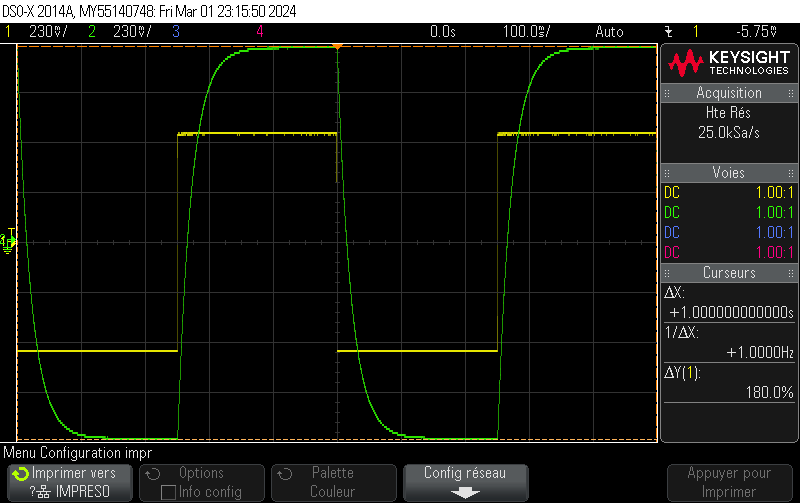
\includegraphics[width=0.75\textwidth]{mesureA1.png}
    \caption{Image de l'oscilloscope lors la mesure de $A$ pour le premiere systeme}
    \label{fig:mesureA1}
\end{figure}

Une fois $A$ connue, sachant que la fréquence de 
coupure a $-3 dB$ $f_{-3dB}$ représente
\[
    20 \cdot log(\left | A \right|) - 3dB =  20 \cdot log\left(\left | A \right|\right) + 20 \cdot log \left( \frac{1}{\sqrt{2}} \right)
    = 20 \cdot log \left( \frac{\left| A \right|}{\sqrt{2}} \right)
\]
on sait qu'on cherche une fréquence pour laquelle l'amplitude de la sortie est $S_{-3dB} \simeq  0.7 \cdot A$, autrement dit $70\%$ de l'amplitude 
dans la bande passante. En connaissant $f_{-3dB}$ on peut commencer a mesurer l'amplification (le rapport sortie / entrée) et le 
déphasage de notre systeme, pour des valeur écarté sur l'échelle logarithmique, mais plus sérré
autour la fréquence $f_{-3dB}$. \par

\begin{figure}[h]
    \centering
    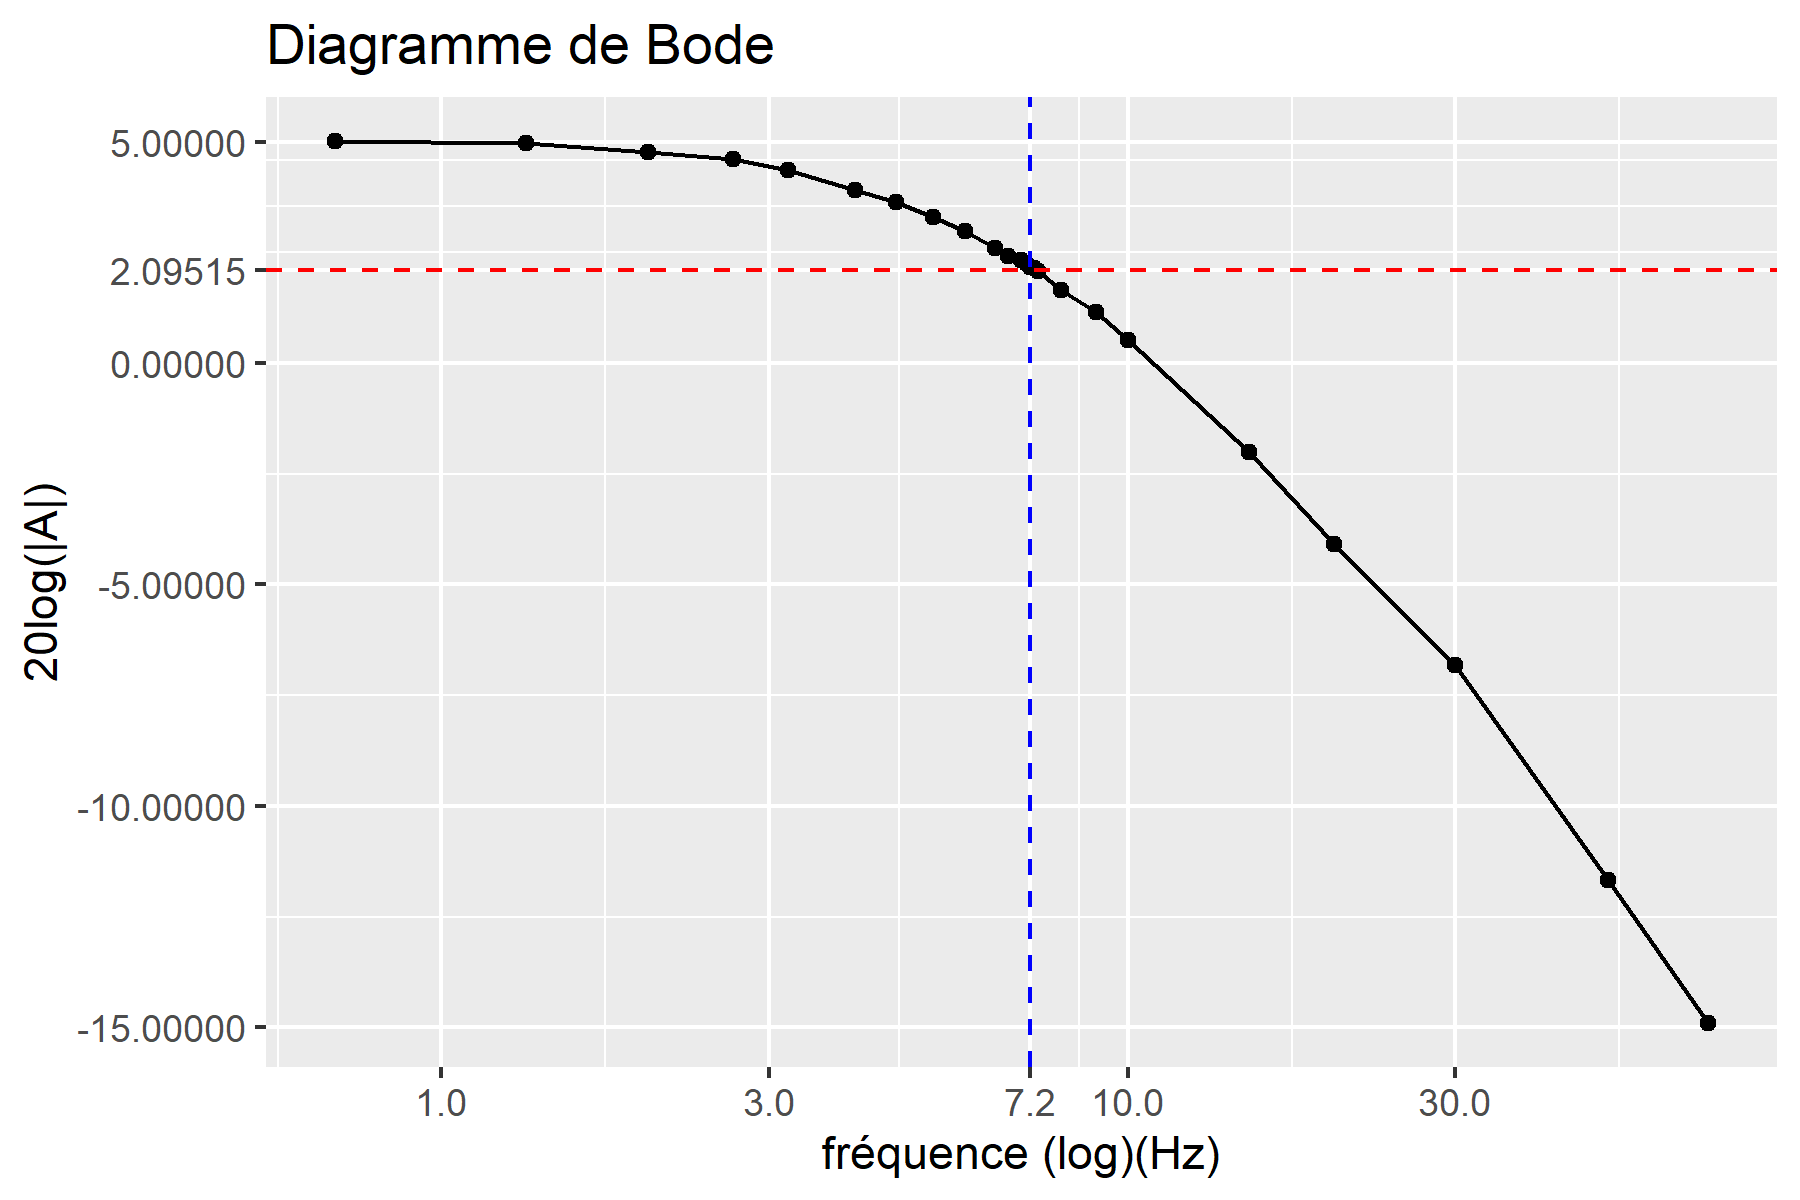
\includegraphics[width=0.75\textwidth]{bode1.png}
    \caption{Diagramme de Bode pour le premiere systeme}
    \label{fig:diagBode1}
\end{figure}

Il est important de noter ici le fait que sur le graphique on a l'impression que
l'intersection des deux droites n'est pas exactement sur la courbe. Il est vrai 
qu'une valeur de $7.4 Hz$ corresponderais mieux sur le graphe pour $f_{-3dB}$ mais 
expérimentalement on a mesuré un déphasage de $-45 \deg$ a une fréquence de $7.2 Hz$, c'est pour 
cela qu'on a décidé de guarder cette valeur.

\begin{figure}[h]
    \centering
    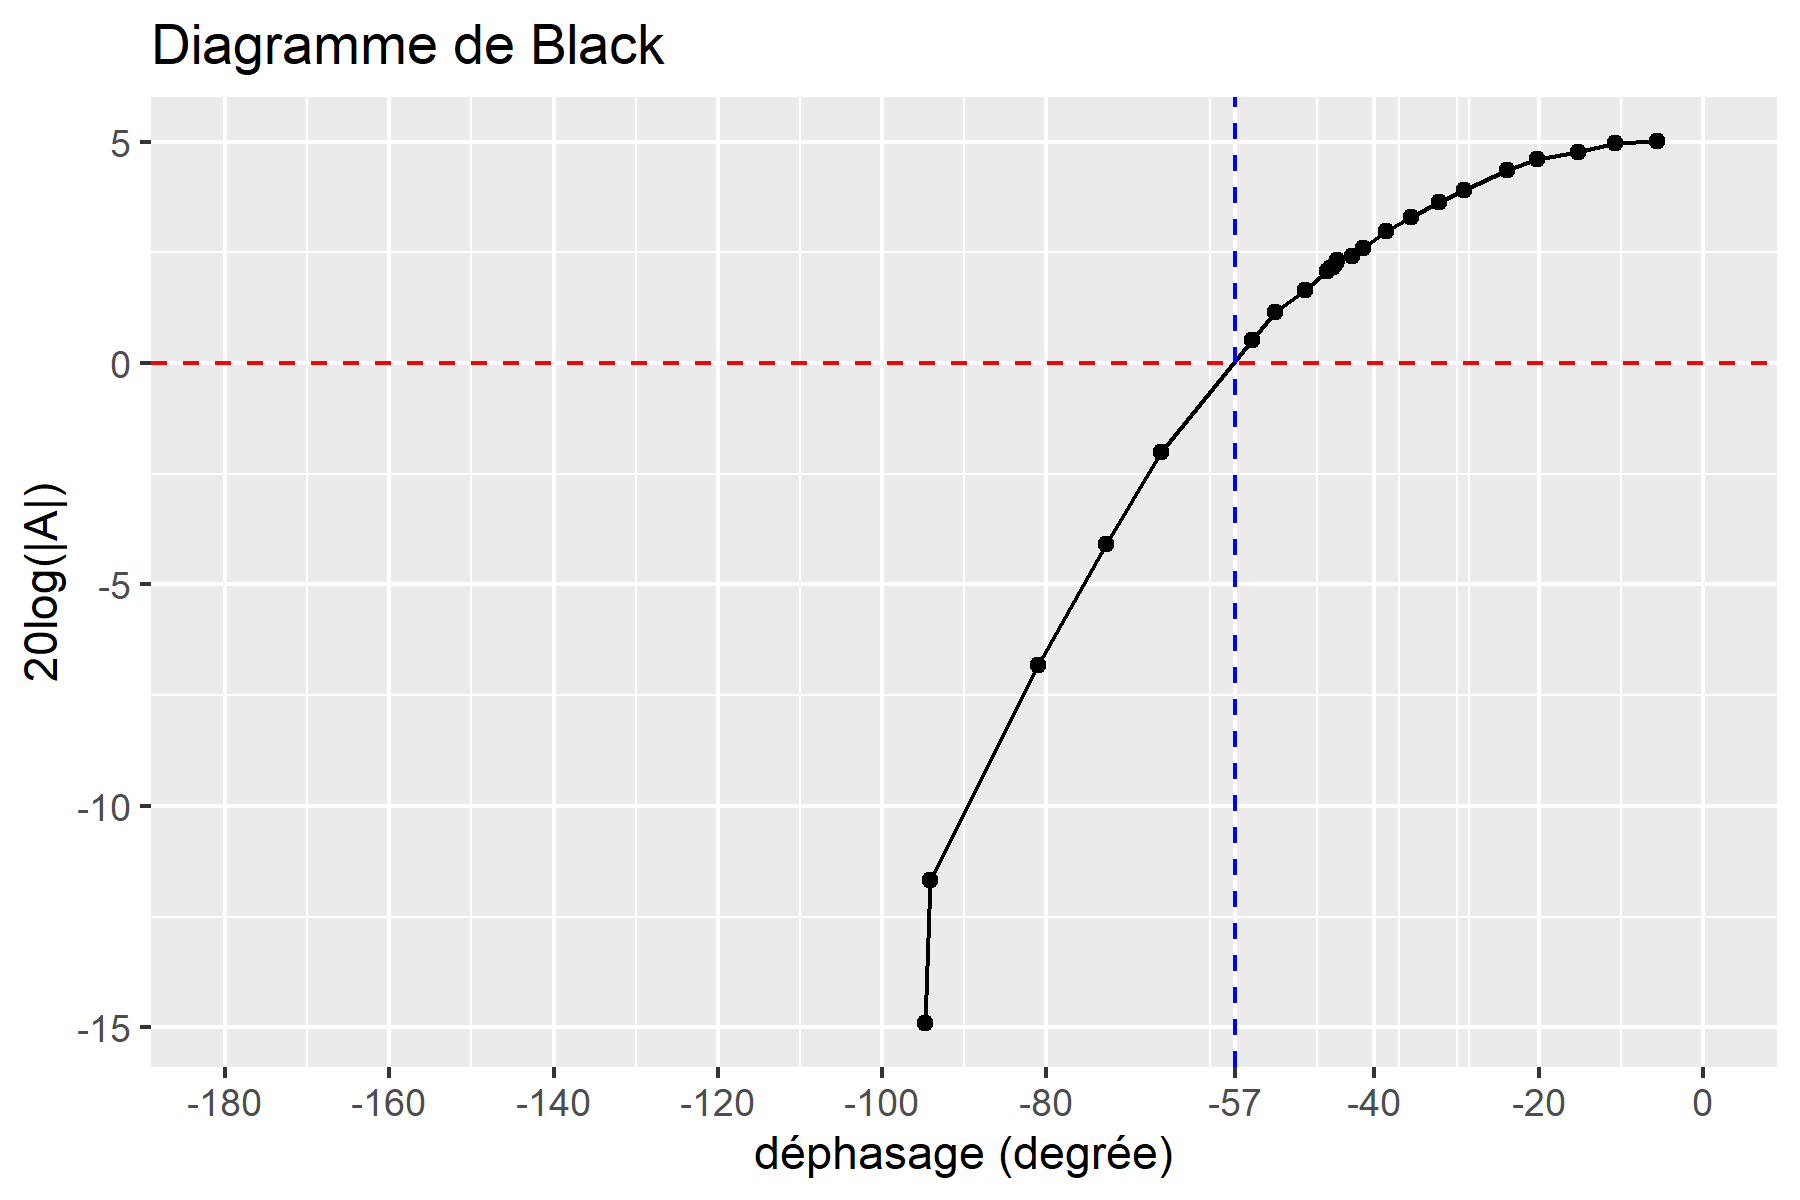
\includegraphics[width=0.75\textwidth]{black1.png}
    \caption{Diagramme de Black pour le premiere systeme}
    \label{fig:diagBlack1}
\end{figure}

Il est possible de déterminer la marge de phase en calculant graphiquement depuis la figure \ref{fig:diagBlack1}, la difference entre 
$-180$ et le point d'intersection de la courbe avec l'axe des abscisses. Dans notre cas:
\[
    M_{ph} = -57 - (-180) = 123 
    \]
La marge de phase est orienté selon les valeurs de l'abscisse croissantes.\par

\subsubsection{Systeme 2}

\section{Réponse indicielle}

\par
Dans cette deuxieme partie on va s'interesser a l'identification des systemes, c'est a dire 
trouver une fonction de transfert, qui décrit au plus proche notre systeme. Il est demandé de tracer
la \textit{caractéristique statique} de notre systeme, qui est la courbe qui représente la sortie
en fonction de l'entrée. Lorsque notre systeme est linéaire, la caractéristique statique est
une droite de pente $A$, l'amplification . En réalité étant donné que le domaine linéaire de la caractéristique statique est
toujours limité (par exemple par la tension de saturation des amplificateurs opérationnelles), c'est a dire 
que la droite n'a pas en tant que limite en $\pm \infty$ l'infini, deux points de cassures, a partir desquelles
la pente devient nulle.
Pour les systemes de premiere ordre de type passe-bas, on peut décrire le systeme dans le domaine de Laplace
par la fonction 
\[
    F_{1}(p) = \frac{A}{1 + \tau p}     
\]
ou $A$ représente l'amplification dans la bande passante (pour les passe-bas c'est aussi\\ l'amplification statique, dans ce cas sans unité)
et $\tau$ le constant de temps. Il est ici possible de déterminer l'amplification $A$ en soumettant notre systeme
a une entrée de type échelon de fréquence $f << 10Hz$. Ceci en realité est faite en mettant un signale carré de fréquence faible. Pour mesurer $\tau$ il suffit de mesurer le temps de réponse a 5 pourcent
c'est a dire le temps a partir duquel la réponse est autour de sa valeur en régime permanent en ne plus dépassant $\pm 5\%$ de cette valeur. On peut bien visualiser
le régime permanent et transitoire au meme temps, si on choisit une fréquence telle que le temps de réponse a $5\%$ est égale a la moitié de la demi-période de notre
signale d'entrée:
\[
    \frac{T_{E}}{4} = t_{5\%}
\]
ou $T_{E}$ est la période du signale d'entrée.
\par
Lorsqu'on souhaite de mesurer ces caractéristiques avec un entrée harmonique (sinusoidale) on peut soumettre le systeme
a un signale sinusoidale de fréquence basse, et on mesure le rapport des valeurs maximums des allures des sortie par rapport a 
l'entrée. Pour trouver $\tau$ on peut mesurer la fréquence de coupure a $-3dB$ en sachant que 
$f_{-3dB} = 2 \pi \omega_{0}$ donc
\[
    \omega_{0} = \frac{f_{-3dB}}{2 \pi}
\]
Il est maintenant facile a déterminer $\tau$ en connaissant la relation
\[
    \tau = \frac{1}{\omega_{0}}
\]
ou $\omega_{0}$ est la pulsation de cassure a $-3dB$ et aussi la pulsation de coupure vu qu'il s'agit 
d'un systeme du premiere ordre.


\end{document}